Zastanawiałeś/aś się kiedyś w środku nocy, ile maksymalnie krawędzi może mieć graf na \(n\) wierzchołkach wolny od kliki rozmiaru \(r\)? Nie? To dobrze świadczy o Twoim zdrowiu psychicznym, ale teraz niestety będziemy musieli sobie to porozważać. Sorki.
\subsection{Graf Turana}
Na początku fajnie byłoby wiedzieć, czym jest graf Turana. Otóż graf Turana \(T_{r-1}(n)\) jest to graf \(r-1\)-dzielny na \(n\) wierzchołkach. Innymi słowy, dzielimy sobie a graf na \(r-1\) grupek (\(A_1, A_2, A_3, \dots\)). Żądamy ponadto, by dla dowolnych \(i,j\) \(|A_i - A_j| \leq 1\). Innymi słowy, chcemy by te ,,grupki'' były zrównoważone. W obrębie danej grupki nie ma krawędzi między wierzchołkami, ale poza tym to wierzchołek z jakiejś grupki łączy się ze wszystkimi pozostałymi wierzchołkami z wszystkich innych grupek. Można o tym myśleć trochę jak o bardziej ogólnej klice dwudzielnej. W sumie to \(T_{2}(2t)\) będzie izomorficzne z kliką dwudzielną \(K_{t,t}\). Zauważmy, że \(T_{r-1}(n)\) na pewno jest wolny od kliki na \(r\) wierzchołkach (to będzie ważne).

\begin{figure}[H]
	\centering
	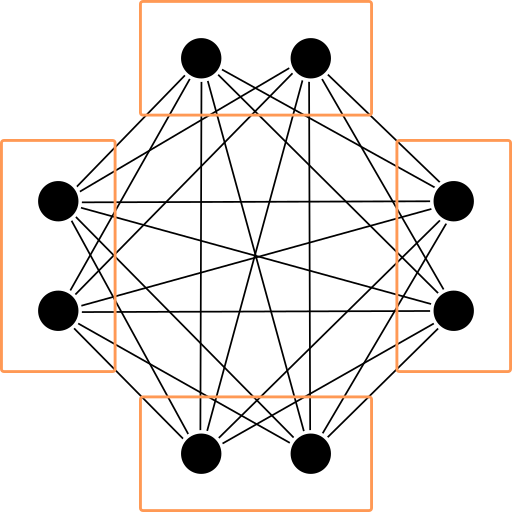
\includegraphics{images/T_3_8.png}
	\caption{Graf \(T_{4}(8)\)}
\end{figure}
\subsection{Twierdzenie Turana}
\begin{theorem}[Turana]
	Dla dowolnego grafu \(G\) o \(n\) wierzchołkach, wolnego od kliki na \(r\) wierzchołkach zachodzi:
	\begin{enumerate}
		\item \(|E(G)| \leq |E(T_{r-1}(n))|\)
		\item Jeśli \(|E(G)| = |E(T_{r-1}(n))|\), to graf \(G\) jest izomorficzny z grafem \(T_{r-1}(n)\).
	\end{enumerate}
\end{theorem}
\begin{proof}
	Uwaga, formaliści się ucieszą bo będę żonglować dziwnymi słowami. Zdefiniujemy sobie \textit{relację} \(R\), taką że para wierzchołków grafu \(G\) \((v_1, v_2) \in R\) jeżeli nie istnieje krawędź między \(v_1\) a \(v_2\). Po co nam ta relacja? Okazuje się, że w grafach Turana relacja ta jest relacją równoważności (co w sumie jest oczywiste; nie masz wierzchołka tylko do innych wierzchołków ze swojej ,,grupki'' -- innymi słowy, każda klasa równoważności stanowi oddzielną ,,grupkę'' grafu Turana, mam nadzieję, że to widać).

	No i jak sobie pomyślimy o tym to jeśli w grafie relacja ta jest relacją równoważności, to jest on prawie grafem Turana. Prawie w tym sensie, że może mieć niezrównoważoną liczbę elementów w grupkach. Jednak za pomocą dowodu \textit{to widać} pokazujemy, że jeśli w grafie tym jest to relacja równoważności, to albo jest izomorficzny z grafem Turana albo można go ,,ulepszyć'', balansując grupki (a więc teza jest spełniona w tym przypadku). Nie, serio, to jest koniec dowodu w tym przypadku, nic formalniejsze nie było wyłożone.

	Co robimy gdy w grafie \(G\) ta relacja nie jest relacją równoważności? Okazuje się, że możemy ją ,,naprawić'', tak, żeby się nią stała (jednocześnie zwiększając liczbę krawędzi, co doprowadzi nas do konkluzji że teza jest prawdziwa). Zauważmy, że jedyne co może się ,,popsuć'' to tranzytywność (ta relacja zawsze będzie symetryczna i zwrotna). Weźmy sobie jakiś przykład wierzchołków, które w takim razie naruszają tranzytywność. Nazwijmy je \(x, y\) i \(z\). Załóżmy, że między \(y\) i \(z\) jest krawędź, ale \(x\) nie ma krawędzi ani do \(y\) ani do \(z\). Załóżmy też BSO, że \(N(y) \geq N(z)\).
	\begin{figure}[H]
		\centering
		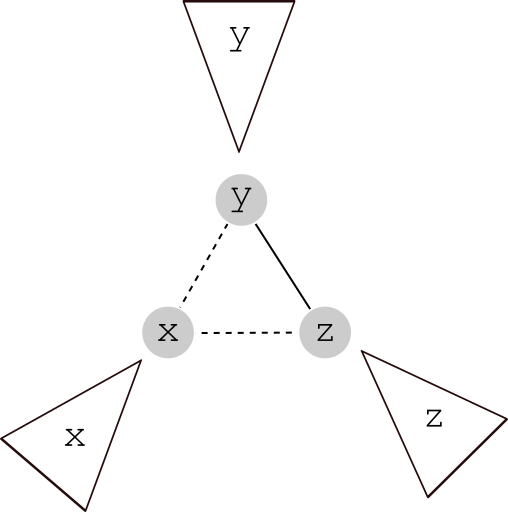
\includegraphics[scale=0.5]{images/turan_bad_case.png}
		\caption{Przypadek przeczący tranzytywności naszej relacji: \(y\) jest w relacji z \(x\) i \(x\) w relacji z \(z\), ale \(y\) nie jest w relacji z \(z\) (bo między \(y\) i \(z\) jest krawędź)}
	\end{figure}
	Rozważmy teraz 2 przypadki:
	\begin{enumerate}
		\item \(|N(x)| > |N(y) \setminus \{z\}|\): Żeby ,,naprawić'' relację, w miejsce \(y\) i \(z\) po prostu wstawiamy ,,kopie'' \(x\), tzn. wierzchołki które łączą się z tymi samymi wierzchołkami z którymi łączy się \(x\). Między \(x\) a jego nowopowstałymi kopiami nie ma żadnych krawędzi. Jako, że \(|N(x)| > |N(y) \setminus \{z\}| \geq |N(z) \setminus \{y\}|\) mamy, że w wyniku tego zabiegu do grafu zostały dodane co najmniej 2 krawędzie, a usunięta została jedna (ta, która łączyła \(y\) i \(z\)). Tym samym naprawiliśmy tranzytywność i zwiększyliśmy liczbę krawędzi, czyli wszystko jest spoko (jednocześnie należy zauważyć, że na pewno nie zwiększyliśmy rozmiaru największej kliki w grafie, bo \(x\) i jego kopie nie są połączone).
		      \begin{figure}[H]
			      \centering
			      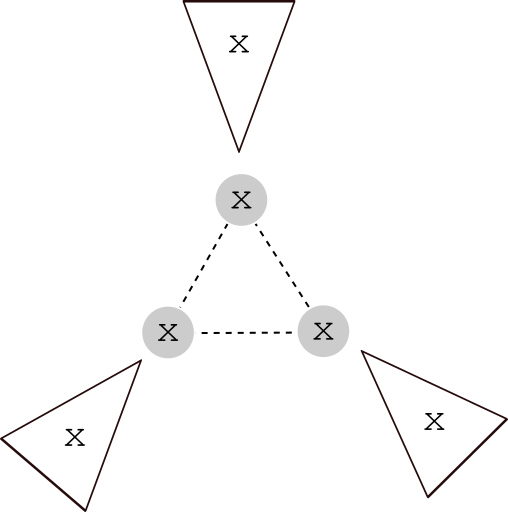
\includegraphics[scale=0.5]{images/turan_case_1.png}
			      \caption{Zamieniliśmy \(y\) i \(z\) na ,,kopie \(x\)''. Jednocześnie usunęliśmy krawędź między \(y\) i \(z\).}
		      \end{figure}

		\item \(|N(x)| \leq |N(y) \setminus \{z\}|\): Robimy tutaj podobnego fikołka jak powyżej, ale tym razem ,,zamieniamy'' \(x\) na \(y\) oraz łączymy kopię \(y\) (czyli to co było wcześniej \(x\)) z \(z\). W ten oto sposób tranzytywność dla tej trójki jest już okej i zwiększyliśmy liczbę krawędzi o co najmniej jedną. Jednocześnie nie zmieniliśmy rozmiaru największej kliki w grafie, bo między \(y\) a jego kopią nie ma krawędzi. \textit{To widać.}

		      \begin{figure}[H]
			      \centering
			      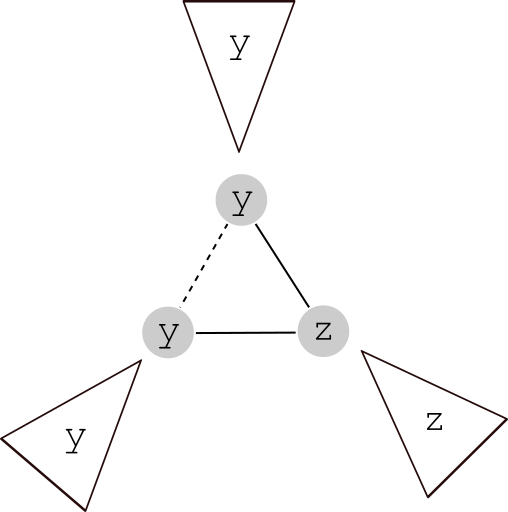
\includegraphics[scale=0.5]{images/turan_case_2.png}
			      \caption{Zamieniliśmy \(x\) ,,kopię \(y\)''. Jednocześnie dodaliśmy krawędź między \(x\) i \(z\).}
		      \end{figure}
	\end{enumerate}
	No i to jest koniec dowodu, bo pokazaliśmy że jak relacja równoważności nie zachodzi to możemy zwiększyć liczbę krawędzi, doprowadzając graf do grafu Turana. Ale fajne.
\end{proof}
